\section{外出先で始めるオレオレストリーミングサーバ}

\subsection{まず}
 どうも。最近はゲーム機向けアプリを作ってる vmatsuoka です。いやー、外でムフフな動画見たいことってありますよねー。今日はそんな要望にお答えするソリューションをご提供します!

\subsection{はじめに}
 最近はスマートフォンなどの携帯端末が普及し、様々な場所で色々な使い方をすることがあると思います。その中でも、スマフォで動画視聴を行うユーザーは多いのではないかと思います。例えば、移動中の暇な時間に動画を視聴したり、家の中でも近くにTV等がない場合にスマフォで視聴することは多いと思います。

 スマフォで動画視聴を行う方法は幾つかあります。スマフォ本体に動画を転送し再生する方法と、ネットワーク経由で動画をストリーミング視聴する方法があります。スマフォ本体に動画を転送する場合は快適な動画視聴を行えますが、本体に保存できる動画に限りがあるので、大量の動画を視聴するのは難しくなります。ネットワーク経由であれば、サーバーに大量の動画を保存することができるので、好きな時に好きな動画を見るといったことが可能になります。本記事ではスマフォでの動画視聴、特に iPhone でネットワーク経由で動画視聴する場合の技術について紹介したいと思います。

 iPhone でネットワーク経由で動画を視聴するには HTTP サーバ上に直接 mp4 を設置し再生する方法と、HTTP Live Streaming(HLS) 方式を用い動画視聴する方法が用意されています。サーバ上に mp4 を直接設置し再生を行う場合は、手軽に構築でき便利です。動画のシークも RangeRequest を用いることで実現でき、快適に視聴できます。しかし、ネットワークのビットレートが動画ビットレートに満たない場合は快適に視聴することは難しくなります。

 対して HLS 方式による再生は直接 mp4 を設置する方法に比べるとサーバー環境を整えるのに手間がかかるものの、ネットワーク帯域にあわせて再生する動画を動的に切り替えたり、動画再生のみではなくライブストリーミングにも対応できるという点でメリットがあります。特に、ネットワーク帯域に合わせて動画を動的に切り替える機能は、外出先等で 3G 回線経由で動画を再生する場合など、ネットワークが不安定な場合にとても有用になります。また、iOS アプリ開発を行う場合、Apple の規約により、HLS の利用が必要な場合があります。

\subsection{HLS 配信方式の特徴}
 映像を配信する手法はいくつか存在します。よく知られているものとして、Adobe の RTMP があります。Youtube などで Flash を利用し動画を視聴する場合に利用されています。RTMP は仕様が公開されているものの標準化はされていなかったり、高機能なため仕組みが比較的複雑になっていたりします。HLS 配信方式は RTMP 同様、動画をストリーミング配信するための方式です。Apple により開発され、標準化を目指して現在はドラフト版が公開されています。仕組みも単純で、要素技術も既に普及したものを利用しているため、わかりやすいものとなっています。HLS では RTMP 同様、VOD と Live Streaming 両方をサポートしています。既にある mp4 を HLS 経由で視聴することや、生放送等をリアルタイムに視聴することができます。

 HLS はデータの配信を HTTP 経由で行なっているため、HTTP サーバに動画コンテンツを設置するだけで対応可能になり、とても手軽に配信を行うことができます。Live Streaming でも同様に逐次配信される動画データを HTTP サーバ上に蓄積していくことで、リアルタイム配信を可能にしています。こういった仕組みはわかりやすく、利用しやすいものとなっています。

 このように HTTP による配信を行なっているのにもかかわらず、回線の帯域に合わせて最適な動画を動的に切り替えるといった機能も持っています。これは、HTTP サーバ上に帯域別の動画を幾つか用意し、動画プレーヤ側で再生する動画を切り替えることで実現しています。HTTP サーバ側では特に特別な処理を行う必要はなく、簡単にマルチビットレート対応が行えることになります。

 こういった機能を実現する仕組みは、動画ファイルを数秒ごとに MPEG2-TS ファイルに変換分割し、プレーヤは TS ファイル単位で取得、再生するという仕組みにより実現されます。MPEG2-TS 形式は地上波デジタル等でも使われている形式で、マルチメディアデータを転送するのに適した形式となっています。サーバ側では変換された TS ファイルとその再生順序を決める m3u8 プレイリストファイルを設置するのみで、プレーヤ側で再生すべきファイルを決定し再生を行う形となっています。したがって、サーバ側に特別な機構は必要なく、HTTP サーバのみがあれば動画配信可能となります。

 さらに、コンテンツの暗号化の対応も簡単で、単に HTTPS 経由でコンテンツを配信するだけで、コンテンツ自体の暗号化を実現できます。HTTPS が利用できない環境向けに、コンテンツそのものを暗号化する仕組みも用意されています。

\subsection{HLS 配信方法}
 ここでは、動画 mp4 ファイルを HLS 方式を用い配信する方法を示したいと思います。
 まず、mp4 ファイルを数秒間隔で分離し、MPEG2-TS ファイルに詰め替えます。Apple が配布してる開発者用ツールなどを用いることで分離することができます。変換分割作業では、再エンコードを行わないので、高速に処理されます。ここで、分割する単位は数秒から10秒程度が推奨されますが、分割可能位置は元動画のキーフレームの入り方に依存してしまうため、目標の間隔で分離できない場合があります。キーフレーム単位で分割するのは、分割後の TS ファイルが単体で再生出来るようにするためです。このような分割を行うことで、シーク等を実現しています。もし、キーフレームが入っていない動画の場合は再エンコードを行いキーフレームを挿入した動画を作成する必要があります。また、マルチビットレートに対応するためにはビットレートの異なる mp4 を用意し、同様に変換分離する必要があります。この時に、それぞれの mp4 のキーフレームの入り方が異なると、シークしたり、ビットレートが切り替わった際に再生位置がずれたりしてしまうので注意が必要です。

 TS ファイルの変換分割が完了したら、分割した TS ファイルの m3u8 プレイリストの作成を行います。プレーヤはこの m3u8 の再生順にしたがって TS ファイルの再生を行います。マルチビットレートに対応する場合は、m3u8 ファイルにビットレートの異なる別の m3u8 ファイルを指定して、プレーヤに教えます。これにより、プレーヤ側では適切なビットレートの動画を選択、再生することが可能になります。

 このようにして用意したファイルを HTTP サーバに設置することで、HLS 配信を実現することができます。

 また、分割変換配信の一連の処理を行なってくれるソリューションが幾つか存在し、wowza media server や Flash Media Server などがよく知られたものになります。これらは mp4 ファイルを設置するのみで、変換や分割、プレイリストの作成を自動的に行い、HLS 配信を行なってくれ手軽に HLS 配信を行うことができます。

\subsection{HLS 配信を行った際に生じた問題}
 実際に HLS 配信を行うにあたって、今回は wowza を利用しました。wowza は mp4 ファイルを自動的に HLS 配信してくれるため、mp4 を事前に変換しておく必要がなく、大量の mp4 を配信しやすくなります。新しく、HLS 配信したい動画があっても、配信用のディレクトリに mp4 を設置するのみで、HLS 配信が可能になります。

 試しに手元の動画を ffmpeg でエンコードし、wowza 経由で HLS 配信してみたところ、問題なく iPhone で視聴することが出来ました。しかし、某動画サイトからダウンロードした mp4 を HLS 配信してみたところ、正常に視聴できないという問題が起こりました。iPhone で視聴すると、最初から連続再生を行う分には問題無いのですが、シークを行ったりすると、映像が切れてしまい、音声のみの再生になってしまうというものです。

 原因を調べてみると、動画中のキーフレームの扱いに問題がある事がわかりました。HLS では TS ファイルに分割する際に、TS ファイルの先頭となるフレームが IDR(Instantaneous Decoder Refresh) フレームであることを要求しています。これは、Apple の HLS 用 Validator でも確認することが出来、問題の mp4 を手動で変換分割したものを Validator でチェックしても、同様に IDR フレームが存在しないという警告が表示されました。

 IDR フレームとはデコーダが IDR フレームに達した時にこれまでのデコード情報を破棄し、それ以降の情報から新たにデコードを開始出来る事を保証するフレームです。H.264 以前のコーデックでは I フレームがキーフレームとなっていて、この位置からデコードを開始すれば正常に映像を構築することが出来ました。しかし、H.264 では I フレームからデコードを開始するのでは映像を正常に構築することができない場合があります。これは、H.264 以前のコーデックが直前のフレームのみを参照するのに対し、H.264 では数フレーム前のフレームを参照することが出来たり、複数フレームを参照することが出来たりするためです。そのため、直前の I フレーム以前のフレームを参照する場合は I フレームからの正常なデコードが保証できなくなりデコードに失敗することになります。そのため、IDR フレームを利用し、IDR フレーム以前の情報を参照しない事をデコーダに伝え、その位置からシークが可能になるようになっています。

 HLS でも TS ファイルに分割する際は、IDR フレーム単位となっており、このような分割をすることで TS ファイル単体で動画を再生することが出来るようになります。そのため、動画のシークも TS ファイル単位で行えることになります。

 問題の動画は IDR フレームが含まれず、TS に分割する際に I フレーム単位で分割されていました。このため iPhone で連続再生する分には問題なくても、シークを行った場合は、映像が正常にデコードできないという状況になります。

 しかし、問題の mp4 を HLS 経由ではなく、mp4 をそのまま再生した場合は何の問題もなく再生やシークを行うことができました。これは、mp4 の状態では I フレームがキーフレームとして機能し、デコードもその位置から開始できていることを示しています。

 問題の mp4 を調べてみると、IDR フレームは含まれていなくても、定期的に I フレームが入っていることが確認できました。さらにこの mp4 では B フレーム(前方、後方参照フレーム)が入っておらず、P フレーム(前方参照フレーム)と I フレームで構成され、前方フレームも直前1フレームのみに設定された動画となっていました。このため I フレームからの再生シークが可能になっているということがわかりました。

 このことから、I フレーム単位で TS ファイルを分割しても、正常にデコードできると考えられますが、実際はそのようにならなかった点は疑問なところとなります。問題の mp4 ファイルでも動画先頭のフレームのみは IDR フレームとなっており、その辺の事情が関係してるのかも知れません。

 問題の mp4 を HLS 配信するには再エンコードを行い IDR フレームが入った mp4 を作成する必要があります。しかし再エンコード作業は動画の数が多いと時間的な面から現実的ではありません。

\begin{center}
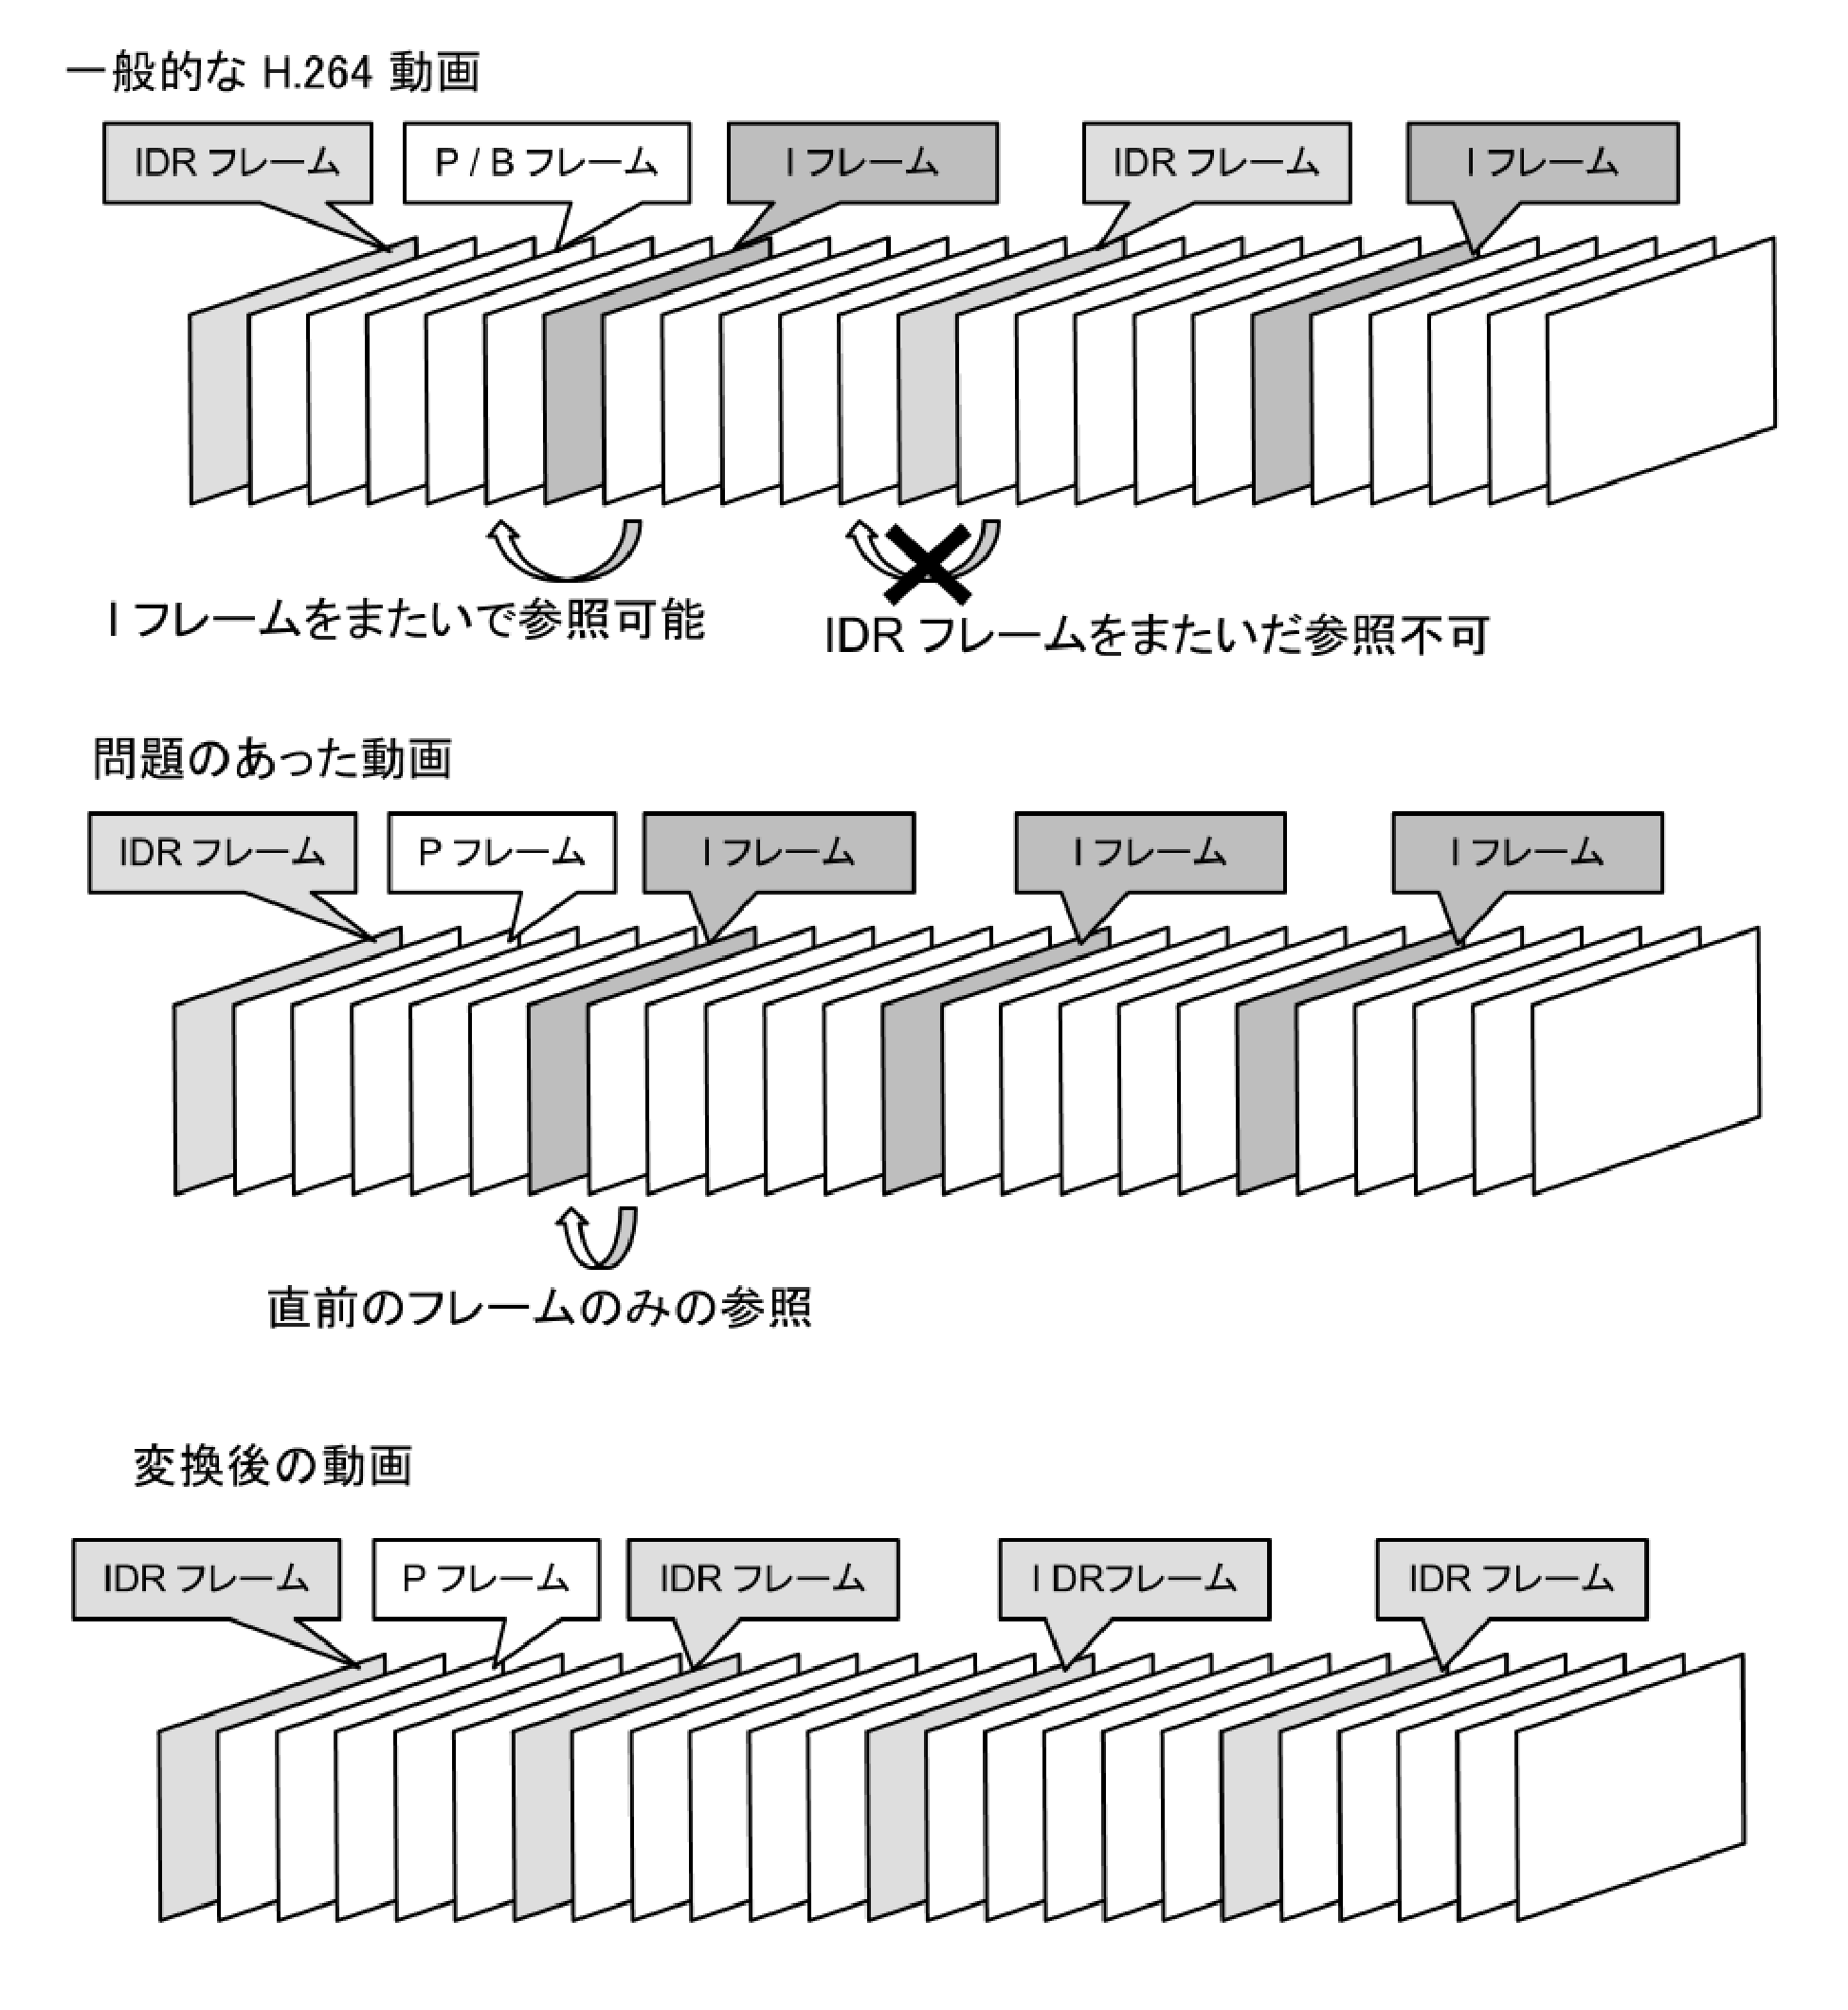
\includegraphics[width=10cm]{vmatsuoka-hls/img/frame.eps}
\end{center}

\subsection{HLS 配信できない動画の変換}
 問題の mp4 すべてを再エンコードするのは現実的ではなかったため、再エンコードせずにうまく解決する方法はないかと探りました。これまでの調査により、動画中のフレームが直前の I フレーム以前の情報を参照しないことはわかっていたため、I フレームを IDR フレームとして扱うことが出来ると考えました。したがって、I フレームを IDR フレームに変換できれば HLS 配信が正常に行えるのではないかと思い、IDR 変換を行なって見ることにしました。

 H.264 仕様を確認してみたところ IDR フレームであることを示すフラグが存在するため、そのフラグを立て、他の部分の整合性を取れば問題ないことがわかりました。Profile の違いにより、フレームのヘッダビット列がある程度変わるものの、Baseline, Main Profile であれば特に大きな変化もないため、対応することができました。IDR 変換作業についても、実際のエンコード情報部分を解釈する必要はなかったため、それほど困難な変換ではありませんでした。

 IDR 変換をかけた動画を再度 HLS 配信してみたところ、今度は正常に視聴ができシーク等も問題ないことが確認できました。一度、動画を作り直す必要は生じてしまいますが、再エンコードするよりは大幅に短い時間で mp4 を準備することが出来るようになり、HLS 経由で視聴でき大変満足です。

\subsection{出典}
\begin{itemize}
\item http://k-tai.impress.co.jp/docs/column/keyword/20120228\_515059.html
\item https://developer.apple.com/jp/devcenter/ios/library/documentation/StreamingMediaGuide.pdf
\item http://en.wikipedia.org/wiki/HTTP\_Live\_Streaming
\item http://tools.ietf.org/html/draft-pantos-http-live-streaming-08
\item http://www.itu.int/rec/T-REC-H.264 H.264 仕様 (ITU-T H.264)
\end{itemize}
